\newcommand{\makeSampleFig}{%
\begin{figure}[tb]
 \centering % avoid the use of \begin{center}...\end{center} and use \centering instead (more compact)
 
\includegraphics[width=\columnwidth]{sample}
 \caption{A visualization of the 1990--2015 data from \autoref{tab:vis_papers}. The image is from \cite{Isenberg:2017:VMC} and is in the public domain.}
 \label{fig:sample}
\end{figure}}

\newcommand{\makeBasicPlottingFig}{%
\begin{figure*}[!htbp]
 \centering
% 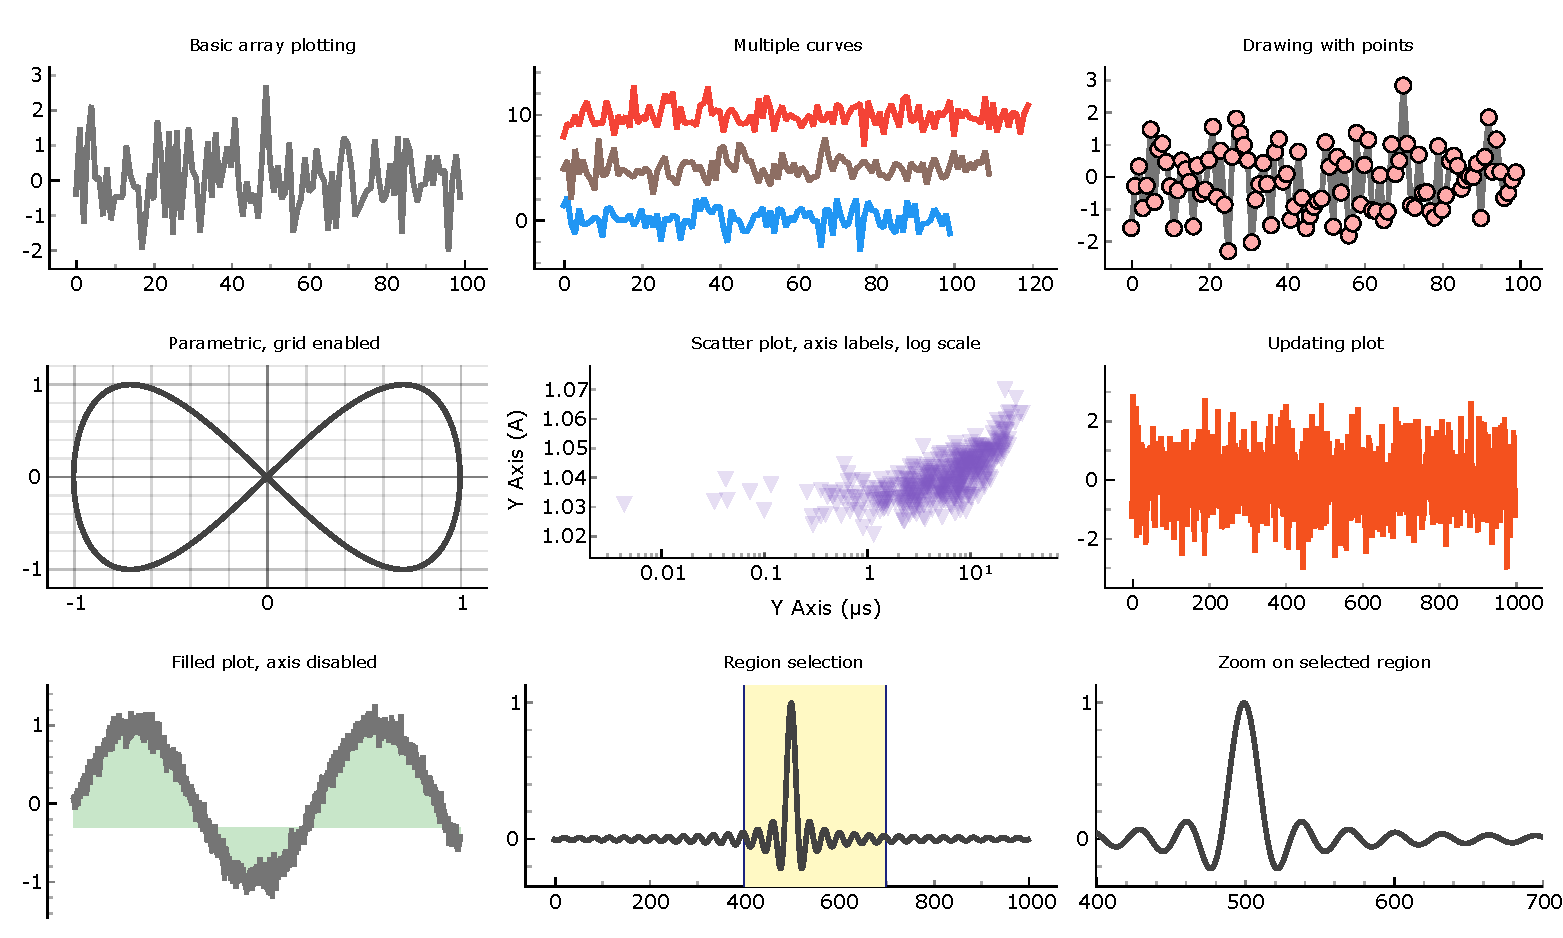
\includegraphics[width=\linewidth]{basicPlotting}
 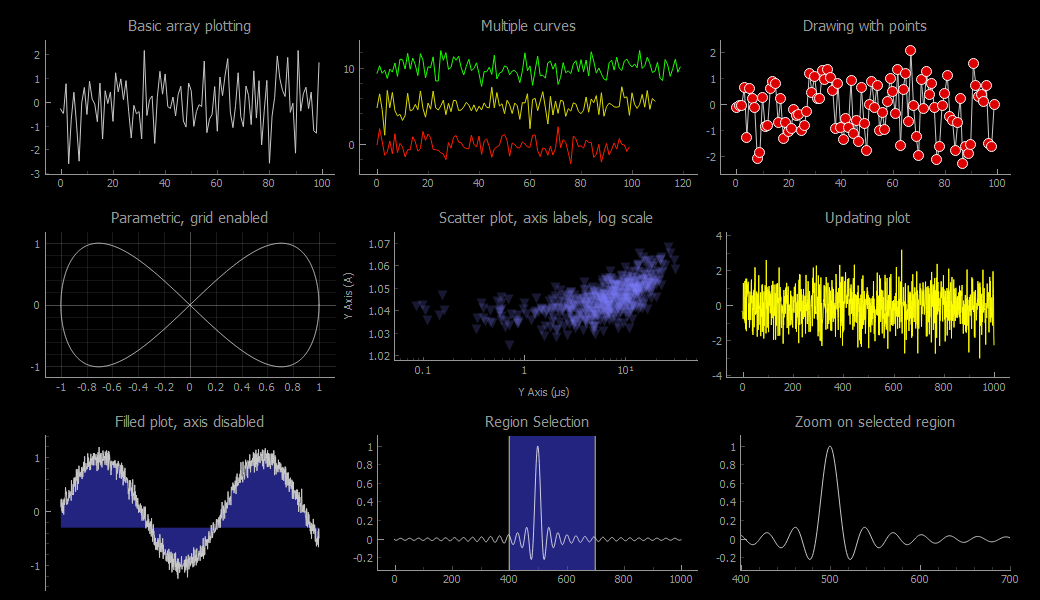
\includegraphics[width=\textwidth]{figures/plotting_example_NN.png}
 \caption{A selection of basic plots from PyQtGraph's suite of examples.}
 \label{fig:basicPlotting}
\end{figure*}}

\newcommand{\makePtreeExFig}{%
\begin{figure}[!htbp]
\centering
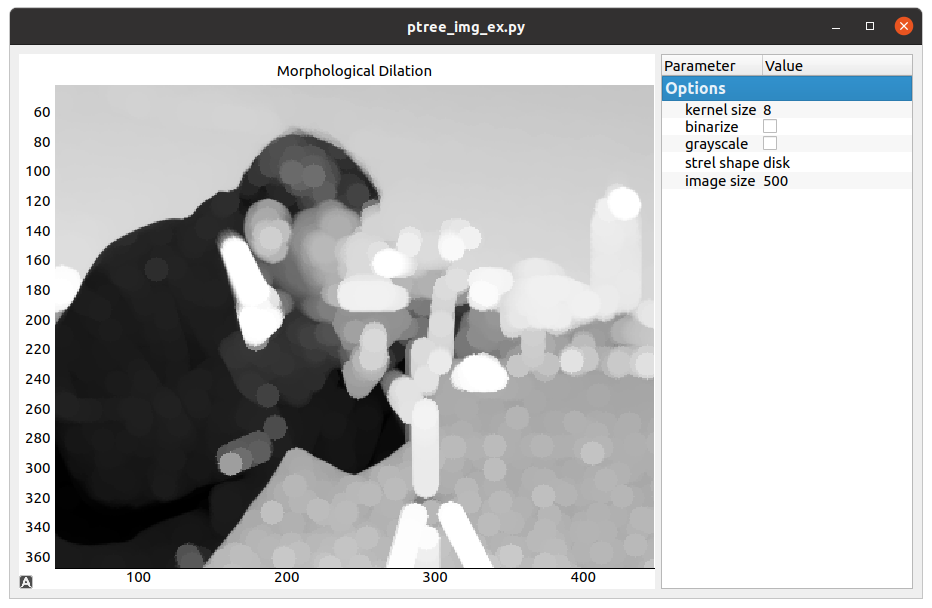
\includegraphics[width=\columnwidth]{figures/pg_ptree_ex}
\caption{Sample use case of parameter trees for function interaction, where various image processing parameters can be quickly updated. Of note, the displayed image reflects these changes in real-time.}
 \label{fig:ptreeEx}
\end{figure}}

\newcommand{\makeMonitoringFig}{%
\begin{figure}[!htbp]
\centering
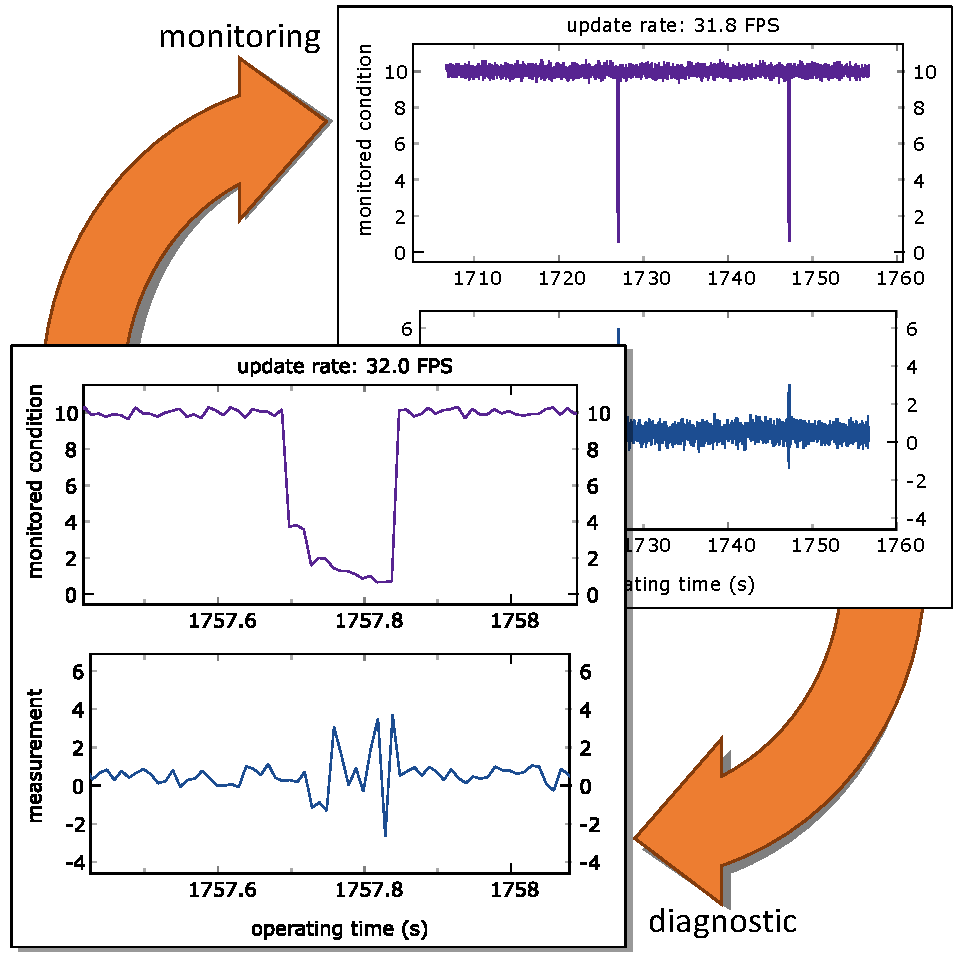
\includegraphics[width=\columnwidth]{figures/monitoring_example_vector.pdf}
\caption{Monitoring and diagnostic of a (simulated) experiment with intermittent failures. Incoming data at 100 samples/s for two measurement channels is recorded into a rolling 5,000 point buffer and continuously displayed at 30 frames/s. When a failure is observed, it can quickly be brought into focus with simple mouse interactions (click-and-drag and mousewheel zoom) for inspection, or to record accurate time stamps. Afterwards, a single click returns the view to automatic scaling without loss of any incoming data.}
 \label{fig:monitoring}
\end{figure}}
